\documentclass[border=4pt]{standalone}
\usepackage{pgfplots}
\pgfplotsset{compat=1.18}

\begin{document}
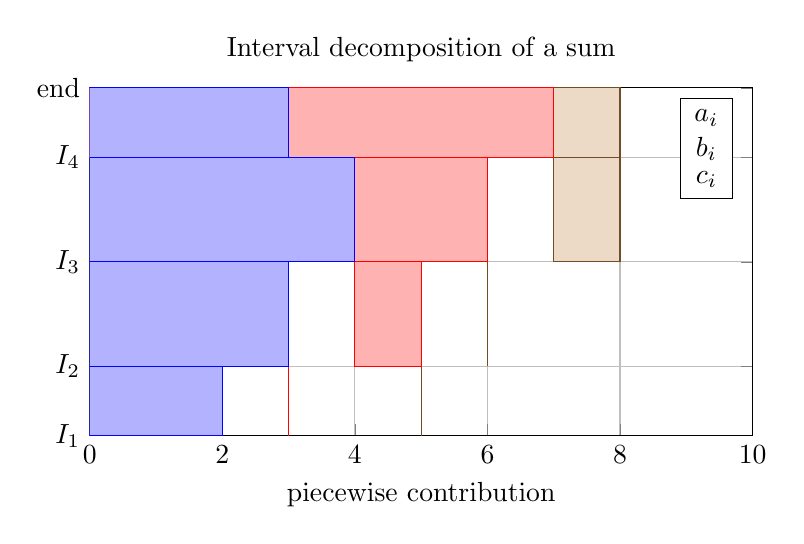
\begin{tikzpicture}
  \begin{axis}[
    xbar interval stacked,
    width=10cm,
    height=6cm,
    xmin=0,
    xmax=10,
    ymin=0,
    ymax=5,
    ytick={0,1,2.5,4,5},
    yticklabels={$I_1$,$I_2$,$I_3$,$I_4$,end},
    xlabel={piecewise contribution},
    title={Interval decomposition of a sum},
    grid=major,
    legend pos=north east
  ]
    \addplot coordinates {(2,0) (3,1) (4,2.5) (3,4) (0,5)};
    \addplot coordinates {(1,0) (2,1) (2,2.5) (4,4) (0,5)};
    \addplot coordinates {(2,0) (1,1) (2,2.5) (1,4) (0,5)};
    \legend{$a_i$,$b_i$,$c_i$}
  \end{axis}
\end{tikzpicture}
\end{document}
